
%% bare_conf.tex
%% V1.3
%% 2007/01/11
%% by Michael Shell
%% See:
%% http://www.michaelshell.org/
%% for current contact information.
%%
%% This is a skeleton file demonstrating the use of IEEEtran.cls
%% (requires IEEEtran.cls version 1.7 or later) with an IEEE conference paper.
%%
%% Support sites:
%% http://www.michaelshell.org/tex/ieeetran/
%% http://www.ctan.org/tex-archive/macros/latex/contrib/IEEEtran/
%% and
%% http://www.ieee.org/

%%*************************************************************************
%% Legal Notice:
%% This code is offered as-is without any warranty either expressed or
%% implied; without even the implied warranty of MERCHANTABILITY or
%% FITNESS FOR A PARTICULAR PURPOSE! 
%% User assumes all risk.
%% In no event shall IEEE or any contributor to this code be liable for
%% any damages or losses, including, but not limited to, incidental,
%% consequential, or any other damages, resulting from the use or misuse
%% of any information contained here.
%%
%% All comments are the opinions of their respective authors and are not
%% necessarily endorsed by the IEEE.
%%
%% This work is distributed under the LaTeX Project Public License (LPPL)
%% ( http://www.latex-project.org/ ) version 1.3, and may be freely used,
%% distributed and modified. A copy of the LPPL, version 1.3, is included
%% in the base LaTeX documentation of all distributions of LaTeX released
%% 2003/12/01 or later.
%% Retain all contribution notices and credits.
%% ** Modified files should be clearly indicated as such, including  **
%% ** renaming them and changing author support contact information. **
%%
%% File list of work: IEEEtran.cls, IEEEtran_HOWTO.pdf, bare_adv.tex,
%%                    bare_conf.tex, bare_jrnl.tex, bare_jrnl_compsoc.tex
%%*************************************************************************

% *** Authors should verify (and, if needed, correct) their LaTeX system  ***
% *** with the testflow diagnostic prior to trusting their LaTeX platform ***
% *** with production work. IEEE's font choices can trigger bugs that do  ***
% *** not appear when using other class files.                            ***
% The testflow support page is at:
% http://www.michaelshell.org/tex/testflow/



% Note that the a4paper option is mainly intended so that authors in
% countries using A4 can easily print to A4 and see how their papers will
% look in print - the typesetting of the document will not typically be
% affected with changes in paper size (but the bottom and side margins will).
% Use the testflow package mentioned above to verify correct handling of
% both paper sizes by the user's LaTeX system.
%
% Also note that the "draftcls" or "draftclsnofoot", not "draft", option
% should be used if it is desired that the figures are to be displayed in
% draft mode.
%
\documentclass[conference]{IEEEtran}
% Add the compsoc option for Computer Society conferences.
%
% If IEEEtran.cls has not been installed into the LaTeX system files,
% manually specify the path to it like:
% \documentclass[conference]{../sty/IEEEtran}





% Some very useful LaTeX packages include:
% (uncomment the ones you want to load)


% *** MISC UTILITY PACKAGES ***
%
%\usepackage{ifpdf}
% Heiko Oberdiek's ifpdf.sty is very useful if you need conditional
% compilation based on whether the output is pdf or dvi.
% usage:
% \ifpdf
%   % pdf code
% \else
%   % dvi code
% \fi
% The latest version of ifpdf.sty can be obtained from:
% http://www.ctan.org/tex-archive/macros/latex/contrib/oberdiek/
% Also, note that IEEEtran.cls V1.7 and later provides a builtin
% \ifCLASSINFOpdf conditional that works the same way.
% When switching from latex to pdflatex and vice-versa, the compiler may
% have to be run twice to clear warning/error messages.






% *** CITATION PACKAGES ***
%
%\usepackage{cite}
% cite.sty was written by Donald Arseneau
% V1.6 and later of IEEEtran pre-defines the format of the cite.sty package
% \cite{} output to follow that of IEEE. Loading the cite package will
% result in citation numbers being automatically sorted and properly
% "compressed/ranged". e.g., [1], [9], [2], [7], [5], [6] without using
% cite.sty will become [1], [2], [5]--[7], [9] using cite.sty. cite.sty's
% \cite will automatically add leading space, if needed. Use cite.sty's
% noadjust option (cite.sty V3.8 and later) if you want to turn this off.
% cite.sty is already installed on most LaTeX systems. Be sure and use
% version 4.0 (2003-05-27) and later if using hyperref.sty. cite.sty does
% not currently provide for hyperlinked citations.
% The latest version can be obtained at:
% http://www.ctan.org/tex-archive/macros/latex/contrib/cite/
% The documentation is contained in the cite.sty file itself.






% *** GRAPHICS RELATED PACKAGES ***
%
\ifCLASSINFOpdf
   \usepackage[pdftex]{graphicx}
  % declare the path(s) where your graphic files are
  % \graphicspath{{../pdf/}{../jpeg/}}
  % and their extensions so you won't have to specify these with
  % every instance of \includegraphics
  % \DeclareGraphicsExtensions{.pdf,.jpeg,.png}
\else
  % or other class option (dvipsone, dvipdf, if not using dvips). graphicx
  % will default to the driver specified in the system graphics.cfg if no
  % driver is specified.
  % \usepackage[dvips]{graphicx}
  % declare the path(s) where your graphic files are
  % \graphicspath{{../eps/}}
  % and their extensions so you won't have to specify these with
  % every instance of \includegraphics
  % \DeclareGraphicsExtensions{.eps}
\fi
% graphicx was written by David Carlisle and Sebastian Rahtz. It is
% required if you want graphics, photos, etc. graphicx.sty is already
% installed on most LaTeX systems. The latest version and documentation can
% be obtained at: 
% http://www.ctan.org/tex-archive/macros/latex/required/graphics/
% Another good source of documentation is "Using Imported Graphics in
% LaTeX2e" by Keith Reckdahl which can be found as epslatex.ps or
% epslatex.pdf at: http://www.ctan.org/tex-archive/info/
%
% latex, and pdflatex in dvi mode, support graphics in encapsulated
% postscript (.eps) format. pdflatex in pdf mode supports graphics
% in .pdf, .jpeg, .png and .mps (metapost) formats. Users should ensure
% that all non-photo figures use a vector format (.eps, .pdf, .mps) and
% not a bitmapped formats (.jpeg, .png). IEEE frowns on bitmapped formats
% which can result in "jaggedy"/blurry rendering of lines and letters as
% well as large increases in file sizes.
%
% You can find documentation about the pdfTeX application at:
% http://www.tug.org/applications/pdftex





% *** MATH PACKAGES ***
%
%\usepackage[cmex10]{amsmath}
% A popular package from the American Mathematical Society that provides
% many useful and powerful commands for dealing with mathematics. If using
% it, be sure to load this package with the cmex10 option to ensure that
% only type 1 fonts will utilized at all point sizes. Without this option,
% it is possible that some math symbols, particularly those within
% footnotes, will be rendered in bitmap form which will result in a
% document that can not be IEEE Xplore compliant!
%
% Also, note that the amsmath package sets \interdisplaylinepenalty to 10000
% thus preventing page breaks from occurring within multiline equations. Use:
%\interdisplaylinepenalty=2500
% after loading amsmath to restore such page breaks as IEEEtran.cls normally
% does. amsmath.sty is already installed on most LaTeX systems. The latest
% version and documentation can be obtained at:
% http://www.ctan.org/tex-archive/macros/latex/required/amslatex/math/





% *** SPECIALIZED LIST PACKAGES ***
%
%\usepackage{algorithmic}
% algorithmic.sty was written by Peter Williams and Rogerio Brito.
% This package provides an algorithmic environment fo describing algorithms.
% You can use the algorithmic environment in-text or within a figure
% environment to provide for a floating algorithm. Do NOT use the algorithm
% floating environment provided by algorithm.sty (by the same authors) or
% algorithm2e.sty (by Christophe Fiorio) as IEEE does not use dedicated
% algorithm float types and packages that provide these will not provide
% correct IEEE style captions. The latest version and documentation of
% algorithmic.sty can be obtained at:
% http://www.ctan.org/tex-archive/macros/latex/contrib/algorithms/
% There is also a support site at:
% http://algorithms.berlios.de/index.html
% Also of interest may be the (relatively newer and more customizable)
% algorithmicx.sty package by Szasz Janos:
% http://www.ctan.org/tex-archive/macros/latex/contrib/algorithmicx/




% *** ALIGNMENT PACKAGES ***
%
%\usepackage{array}
% Frank Mittelbach's and David Carlisle's array.sty patches and improves
% the standard LaTeX2e array and tabular environments to provide better
% appearance and additional user controls. As the default LaTeX2e table
% generation code is lacking to the point of almost being broken with
% respect to the quality of the end results, all users are strongly
% advised to use an enhanced (at the very least that provided by array.sty)
% set of table tools. array.sty is already installed on most systems. The
% latest version and documentation can be obtained at:
% http://www.ctan.org/tex-archive/macros/latex/required/tools/


%\usepackage{mdwmath}
%\usepackage{mdwtab}
% Also highly recommended is Mark Wooding's extremely powerful MDW tools,
% especially mdwmath.sty and mdwtab.sty which are used to format equations
% and tables, respectively. The MDWtools set is already installed on most
% LaTeX systems. The lastest version and documentation is available at:
% http://www.ctan.org/tex-archive/macros/latex/contrib/mdwtools/


% IEEEtran contains the IEEEeqnarray family of commands that can be used to
% generate multiline equations as well as matrices, tables, etc., of high
% quality.


%\usepackage{eqparbox}
% Also of notable interest is Scott Pakin's eqparbox package for creating
% (automatically sized) equal width boxes - aka "natural width parboxes".
% Available at:
% http://www.ctan.org/tex-archive/macros/latex/contrib/eqparbox/





% *** SUBFIGURE PACKAGES ***
%\usepackage[tight,footnotesize]{subfigure}
% subfigure.sty was written by Steven Douglas Cochran. This package makes it
% easy to put subfigures in your figures. e.g., "Figure 1a and 1b". For IEEE
% work, it is a good idea to load it with the tight package option to reduce
% the amount of white space around the subfigures. subfigure.sty is already
% installed on most LaTeX systems. The latest version and documentation can
% be obtained at:
% http://www.ctan.org/tex-archive/obsolete/macros/latex/contrib/subfigure/
% subfigure.sty has been superceeded by subfig.sty.



%\usepackage[caption=false]{caption}
%\usepackage[font=footnotesize]{subfig}
% subfig.sty, also written by Steven Douglas Cochran, is the modern
% replacement for subfigure.sty. However, subfig.sty requires and
% automatically loads Axel Sommerfeldt's caption.sty which will override
% IEEEtran.cls handling of captions and this will result in nonIEEE style
% figure/table captions. To prevent this problem, be sure and preload
% caption.sty with its "caption=false" package option. This is will preserve
% IEEEtran.cls handing of captions. Version 1.3 (2005/06/28) and later 
% (recommended due to many improvements over 1.2) of subfig.sty supports
% the caption=false option directly:
%\usepackage[caption=false,font=footnotesize]{subfig}
%
% The latest version and documentation can be obtained at:
% http://www.ctan.org/tex-archive/macros/latex/contrib/subfig/
% The latest version and documentation of caption.sty can be obtained at:
% http://www.ctan.org/tex-archive/macros/latex/contrib/caption/




% *** FLOAT PACKAGES ***
%
%\usepackage{fixltx2e}
% fixltx2e, the successor to the earlier fix2col.sty, was written by
% Frank Mittelbach and David Carlisle. This package corrects a few problems
% in the LaTeX2e kernel, the most notable of which is that in current
% LaTeX2e releases, the ordering of single and double column floats is not
% guaranteed to be preserved. Thus, an unpatched LaTeX2e can allow a
% single column figure to be placed prior to an earlier double column
% figure. The latest version and documentation can be found at:
% http://www.ctan.org/tex-archive/macros/latex/base/



%\usepackage{stfloats}
% stfloats.sty was written by Sigitas Tolusis. This package gives LaTeX2e
% the ability to do double column floats at the bottom of the page as well
% as the top. (e.g., "\begin{figure*}[!b]" is not normally possible in
% LaTeX2e). It also provides a command:
%\fnbelowfloat
% to enable the placement of footnotes below bottom floats (the standard
% LaTeX2e kernel puts them above bottom floats). This is an invasive package
% which rewrites many portions of the LaTeX2e float routines. It may not work
% with other packages that modify the LaTeX2e float routines. The latest
% version and documentation can be obtained at:
% http://www.ctan.org/tex-archive/macros/latex/contrib/sttools/
% Documentation is contained in the stfloats.sty comments as well as in the
% presfull.pdf file. Do not use the stfloats baselinefloat ability as IEEE
% does not allow \baselineskip to stretch. Authors submitting work to the
% IEEE should note that IEEE rarely uses double column equations and
% that authors should try to avoid such use. Do not be tempted to use the
% cuted.sty or midfloat.sty packages (also by Sigitas Tolusis) as IEEE does
% not format its papers in such ways.





% *** PDF, URL AND HYPERLINK PACKAGES ***
%
%\usepackage{url}
% url.sty was written by Donald Arseneau. It provides better support for
% handling and breaking URLs. url.sty is already installed on most LaTeX
% systems. The latest version can be obtained at:
% http://www.ctan.org/tex-archive/macros/latex/contrib/misc/
% Read the url.sty source comments for usage information. Basically,
% \url{my_url_here}.





% *** Do not adjust lengths that control margins, column widths, etc. ***
% *** Do not use packages that alter fonts (such as pslatex).         ***
% There should be no need to do such things with IEEEtran.cls V1.6 and later.
% (Unless specifically asked to do so by the journal or conference you plan
% to submit to, of course. )


% correct bad hyphenation here
\hyphenation{op-tical net-works semi-conduc-tor}


\begin{document}
%
% paper title
% can use linebreaks \\ within to get better formatting as desired
\title{Distributed System Report}
%\title{Bare Demo of IEEEtran.cls for Conferences}


% author names and affiliations
% use a multiple column layout for up to three different
% affiliations
\author{
\IEEEauthorblockN{Quang Anh Pham Nguyen}
\IEEEauthorblockA{pnquanganh1986@gmail.com}
\and
\IEEEauthorblockN{Jun Zhang}
\IEEEauthorblockA{jay.z.frozen@gmail.com}
\and
\IEEEauthorblockN{Sibo Wang}
\IEEEauthorblockA{wangsibo.victor@gmail.com}
}
% conference papers do not typically use \thanks and this command
% is locked out in conference mode. If really needed, such as for
% the acknowledgment of grants, issue a \IEEEoverridecommandlockouts
% after \documentclass

% for over three affiliations, or if they all won't fit within the width
% of the page, use this alternative format:
% 
%\author{\IEEEauthorblockN{Michael Shell\IEEEauthorrefmark{1},
%Homer Simpson\IEEEauthorrefmark{2},
%James Kirk\IEEEauthorrefmark{3}, 
%Montgomery Scott\IEEEauthorrefmark{3} and
%Eldon Tyrell\IEEEauthorrefmark{4}}
%\IEEEauthorblockA{\IEEEauthorrefmark{1}School of Electrical and Computer Engineering\\
%Georgia Institute of Technology,
%Atlanta, Georgia 30332--0250\\ Email: see http://www.michaelshell.org/contact.html}
%\IEEEauthorblockA{\IEEEauthorrefmark{2}Twentieth Century Fox, Springfield, USA\\
%Email: homer@thesimpsons.com}
%\IEEEauthorblockA{\IEEEauthorrefmark{3}Starfleet Academy, San Francisco, California 96678-2391\\
%Telephone: (800) 555--1212, Fax: (888) 555--1212}
%\IEEEauthorblockA{\IEEEauthorrefmark{4}Tyrell Inc., 123 Replicant Street, Los Angeles, California 90210--4321}}




% use for special paper notices
%\IEEEspecialpapernotice{(Invited Paper)}




% make the title area
\maketitle


%\begin{abstract}
%\boldmath
%The abstract goes here.
%\end{abstract}
% IEEEtran.cls defaults to using nonbold math in the Abstract.
% This preserves the distinction between vectors and scalars. However,
% if the conference you are submitting to favors bold math in the abstract,
% then you can use LaTeX's standard command \boldmath at the very start
% of the abstract to achieve this. Many IEEE journals/conferences frown on
% math in the abstract anyway.

% no keywords




% For peer review papers, you can put extra information on the cover
% page as needed:
% \ifCLASSOPTIONpeerreview
% \begin{center} \bfseries EDICS Category: 3-BBND \end{center}
% \fi
%
% For peerreview papers, this IEEEtran command inserts a page break and
% creates the second title. It will be ignored for other modes.
\IEEEpeerreviewmaketitle

\section{Architecture}
The design of our system is based on the Google File System\cite{gfs}. Figure (\ref{fig:a}) illustrates the overall architure of our distributed system.
The system consists of a single master, multiple slaves and  multiple clients. Instead of using replicas to prevent from data loss, our system implements erasure code requiring lower storage usage. The master maintains metadata of files stored on this system. The metadata of a file includes: encoded parts of the file, information of slaves storing these parts and the size of the original file. Slaves are responsible for storing data objects sent to them and returning these objects when requested. Each slave periodically sends its state to the master through heartbeat messages to claim that it is alive. The data object stored on the slave corresponds to a file. The encoding/decoding operations are executed on this object. The client can access the system to write and read data.
Clients interact with the master and obtain the metadata of a file. After that, clients can communicate with slaves to get the content of the original file.

\section{Operations}
In this system, read and write operations are the most concerned. Both read and write operations need the coordination of masters and slaves to be finished. The detail of how these two opeations are conducted are given below.
\subsection{Write operation}
A write operation is lanuched by the client, and it mainly includes 3 steps to finish.
\begin{itemize}
\item Request: the client makes a request to the master to notify about this operation. The original size of the file is also included in this request for the decoding step in the future. The master itself records the information as the  metadata  of this file before sending them to the client.
\item Encode data: The client encodes the file into several parts using erasure codes. For example, if we have a file $O$, we will encode it into 7 parts with the hierarcial code, $O1$,$O2$,$O3$,$O4$,$O1O2$,$O3O4$, $O1O2O3O4$.
\item  Write to stable storage: the client contacts to each of slaves on the list and transfers the corresponding file name, part index and encoded data to the slaves. The slave stores this data as a file in its local file system with the name combined from original file name and part index (for example: a.txt.O1, a.txt.O1O2). 
\end{itemize}

However, there may be failures in the communication with the slaves. These failures may be caused by a communication problem or the fact that the slave already died and the master has not known about this (because of the delay in the maintaining process). We assume that there is only second type of failure in our experiments. In that case, the client should ignore these errors because sooner or later the master will detect this dead slave. The client does not need to acknowledge the master about the failed slave, which keeps the system still simple and efficient in failure handling.

\subsection{Read operation}
Similarly, a read operation includes 3 phases.
\begin{itemize}
\item Request: The client requests to the master to obtain the metadata of the file.
\item Obtain Encoded data:  The client determines which slaves it should contact to retrieve the encoded data. For example, to read a file $O$, it has a list of slaves containing $O1$,$O2$,$O3$,$O4$,$O1O2$,$O3O4$, $O1O2O3O4$, the client will choose to communicate with the slaves owning the first 4 encoded data if they are all alive, otherwise, assume the slave owning $O2$ is dead, and in the list there is only information for slaves contain $O1$,$O3$,$O4$,$O1O2$,$O3O4$, $O1O2O3O4$, then the client will choose to communicate with $O1$, $O1O2$,$O3$,$O4$. The client can communicate with each slave sequentially or concurrently for a better performance. 
\item Decode data: the client decodes the data and obtain the  original file content.
\end{itemize}
Similar to the write operation, there may exist a chance of failures because of 2  reasons mentioned above. In both cases, the client has to recalculate to decide one or more other parts needed to recover data; therefore, more communications are required. With these collected pieces of information, the decoding process is executed by the client. If the original file cannot be reconstructed in some fault scenarios, the read operation is unsuccessful. 

\begin{figure}
	\centering
		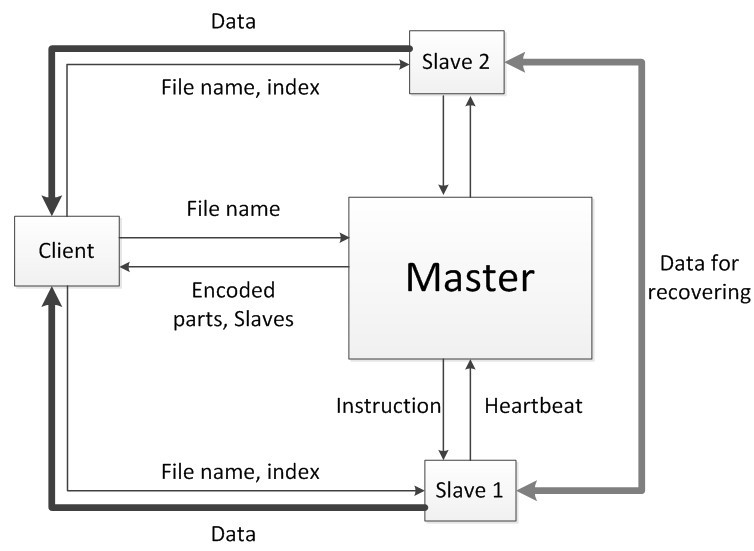
\includegraphics[height=50mm]{a.jpg}
		\caption{System Arcitecture}
	\label{fig:a}
\end{figure}


\section{Failure Handling}
% no \IEEEPARstart
\subsection{Failure Detection}
In our distributed file system, the master maintains a timestamp table to record the last heartbeating time for every registered slave. Slaves are designed to send heartbeat messages to the master every $t_b$ seconds. After receiving the heartbeat message, the master updates the timestamp of that slave to the current system time. On the master side, a thread is built to check the timestamp table every $t_c$ seconds. Once the absolute difference between the timestamp of a slave and current system time of master exceeds a prescribed threshold, the master adds the slave to a \textit{dead\_slave}  list. After checking the timestamp of all slaves, the master starts the recovery process if the \textit{dead\_slave} list is not empty.
\subsection{Data recovery: Master Side}
In the data recovery function, the master first establishes a list containing all damaged files and their damaged part indexes, according to the \textit{dead\_slave} list and the metadata of all files. For each damaged file, the recovery process is given as follows.
\begin{itemize}
\item Input: Damaged indexes set $S$, e.g., $\left\{O2, O1O2, O3O4\right\}$;
\item Initialization: Mark damaged indexes as LOST, and set their recovery set $R$ as empty set (following the example, $O2$ is marked as LOST and $R_{O2} = \emptyset$ ); Mark non-damaged indexes as OK and set their recovery set $R$ to a set containing themselves ($O1$ is OK, and $R_{O1} = \left\{O1\right\}$ meaning O1 can be recovered by itself, or no recovery needed);
\item Bottom-up Recovery Phase: Check indexes in a bottom-up order: $O1, O2, O3, O4, O1O2, O3O4, O1O2O3O4$. If an index $i$ is LOST and both of its children, say $c1$ and $c2$, are OK, mark $i$ as OK and update $R_{i}$ to $R_{c1}\cup R_{c2}$; In our example, $O3O4$ is recovered and $R_{O3O4} = R_{O3}\cup R_{O4} = \left\{O3, O4\right\}$ while $O2$ (no child) and $O1O2$ (child $O2$ is LOST) cannot be restored.
\item Top-down Recovery Phase: Check indexes in a top-down order: $O1O2O3O4, O1O2, O3O4, O1, O2, O3, O4$. If an index $i$ is LOST and both of its father $f$ and sibling $s$ are OK, mark $i$ as OK and update $R_{i}$ to $R_{f}\cup R_{s}$; In our example, $O1O2$ is recovered first by $O1O2O3O4$ and $O3O4$ with $R_{O1O2} = R_{O1O2O3O4}\cup R_{O3O4} = \left\{O3, O4, O1O2O3O4\right\}$. Then $O2$ gets recovered by $O1O2$ and $O1$ with $R_{O2} = R_{O1O2}\cup R_{O1} = \left\{O1, O3, O4, O1O2O3O4\right\}$.
\item Return: If there exists empty $R_i$ for any index $i$, return failed, else return all $R_i$ with $|R_i|\ge2$.
\end{itemize}

If the recovery process returns failed, which means we cannot recover this file by remaining parts, our system delete this file from file list. Otherwise, we assign a new slave (with best-effort distributed law) for each missing index, and call the recovery process at the slave side with input argument: index to recover and a list of $(index, slave)$ pair for every needed index. 


\subsection{Data recovery: Slave Side}
Upon receiving the recovery request from the master, the slave obtain the missing index for the damaged file and know where to obtain the needed indexes to recover the missing index with the help of input arguments. Afterwards, the slave do the recovery with the following steps:
\begin{itemize}
\item Obtain indexes for recovery: The recovery slave read needed index from the slave which owns the index for the preparation of recovery. Here, the recovery slave acts like a client, and do a read operation from the slave who owns the index. For example, if the input argument is $O3O4$, and $<(O3,slave2),(O4,slave3)>$, the recovery slave will do a read operation to $O3$ from slave2, and a read opeartion to $O4$ from slave3 for the preparation of recovery index $O3O4$.
\item Recovery data: After obtaining the indexes needed to recover the missing index, the recovery slave do the encode process for the indexes read in the previous step. For the example in previous step, the recovery slave is able to  encode for $O3O4$ with the content of index $O3$ and $O4$. After encoding, we obtain the content of index $O3O4$.
\item Write to stable storage: The recovery slave write the content of missing index into its local disk and finish the recovery process for this missing index.
\end{itemize}
If there are many recovery requests from the master, the slave will do recovery for missing indexes one by one until it finishes all of the recovery request. When the slave doing recovery, it will not block the read and write requests from clients. 



\subsection{Fault tolerance}
If only one slave is dead, the client is still able to reconstruct the original file. However, when the number of dead slaves is more than 2, there are certain files cannot be recovered. This happens in one the following cases:
\begin{itemize}
\item The O1 and O2 parts are lost at the same time (the same for O3 and O4).
\item	One of the parts O1, O2, O3 and O4 is lost and it cannot be recovered from the higher-layered parts (O1O2, O3O4 and O1O2O3O4).
\end{itemize}
In both cases, the system is not able to reconstruct one or more parts of O1, O2, O3 and O4 from the remaining data; therefore, it cannot rebuild the original file. Because the master asked the client to write 7 encoded pieces of Hierarchical code instance into different 7 slaves, both failed situations happen only when more than one slave is down. As the number of dead slave increases, the chance for these cases also increases; hence, more files are not able to be recovered

\section{Cost analyses}
\subsection{Reading Cost}
When reading a file with the size S, the client tries to read the parts in {O1, O2, O3, O4} first. If there are not any errors in this step, the client has to perform 5 requests: 1 to master for Metadata and 4 to each slave. If the requests to slaves are executed sequentially, the total delay of a read operation is 5 round trips as well. However, the client can read data from slaves concurrently and in this case the total delay is only 2 round trips. The bandwidth consumed in a read operation is S (assume that the size of Metadata is not considerable compared to S).

When the client cannot retrieve one of the parts of in {O1, O2, O3, O4}, say O1, it has to get the O1O2 and O3O4, O1O2O3O4 if necessary. Because slaves send heart beat messages to master every tb seconds, there is a latency when the master discovers the dead node and repair the lost data in that node. In this period of time, the master still returns the location of dead slaves to the client and the client will find out the state of these nodes after requesting to them. Hence, the client will consume one more request for each unknown dead slave. In our example, the client has to get the O1O2 piece to recreate the O1, the delay will increase by 1 round trip, the used bandwidth is 5/4 S. If the master knows that the O1O2 part is missing (and does not include this part in the list returned to client), the client will request to get O3O4 and O1O2O3O4; in this case, the delay will be added by 2 round trips and the total bandwidth consumed is  3/2 S. In the worst case, the master has not found that one or both two parts of O1O2 and O1O2O3O4 are not available; the client may waste up to 6 or 7 requests and the total bandwidth will be 3/2 S and 7/4 S, respectively.


\subsection{Repairing Cost}
Similar to the read operation, the repair delay depends on the number of data pieces to recover the lost piece. To recover the O1 the system spends 3 requests: 1 from master to the slave which will store O1; and 2 from this slave to acquire O2, O1O2. The delay will be 2 roundtrips if the last 2 requests are executed concurrently and the bandwidth is 1/2 S. In general, if we have to read n parts to recover one data piece, the delay is always 2 round trips and the consumed bandwidth is  n/4 S.

\section{Lessons}
In the process of designing, implementing and testing the system, we learned several useful lessons.
One lesson we learned is that it is important to break the system into modules interacting via carefully designed interfaces. By clearly defining modules with specific tasks and actions, our team can develop each module independently and it takes little time and efforts to integrate these parts together. It does not only save the development time but also makes it easier to debug.
Another lesson that we learned is the importance of applying RPC in distributed systems. In this project, we mainly focus on architecture-level aspects and we do not want to spend a lot of time on dealing with communication matters such as connection managing, object serializing and deserializing, error handling, etc. That is the reason why we use Java RMI to hide the details of communication implementation and make our system as simple as possible.


%This demo file is intended to serve as a ``starter file''
%for IEEE conference papers produced under \LaTeX\ using
%IEEEtran.cls version 1.7 and later.
% You must have at least 2 lines in the paragraph with the drop letter
% (should never be an issue)
%I wish you the best of success.

%\hfill mds
 
%\hfill January 11, 2007

%\subsection{Subsection Heading Here}
%Subsection text here.


%\subsubsection{Subsubsection Heading Here}
%Subsubsection text here.


% An example of a floating figure using the graphicx package.
% Note that \label must occur AFTER (or within) \caption.
% For figures, \caption should occur after the \includegraphics.
% Note that IEEEtran v1.7 and later has special internal code that
% is designed to preserve the operation of \label within \caption
% even when the captionsoff option is in effect. However, because
% of issues like this, it may be the safest practice to put all your
% \label just after \caption rather than within \caption{}.
%
% Reminder: the "draftcls" or "draftclsnofoot", not "draft", class
% option should be used if it is desired that the figures are to be
% displayed while in draft mode.
%
%\begin{figure}[!t]
%\centering
%\includegraphics[width=2.5in]{myfigure}
% where an .eps filename suffix will be assumed under latex, 
% and a .pdf suffix will be assumed for pdflatex; or what has been declared
% via \DeclareGraphicsExtensions.
%\caption{Simulation Results}
%\label{fig_sim}
%\end{figure}

% Note that IEEE typically puts floats only at the top, even when this
% results in a large percentage of a column being occupied by floats.


% An example of a double column floating figure using two subfigures.
% (The subfig.sty package must be loaded for this to work.)
% The subfigure \label commands are set within each subfloat command, the
% \label for the overall figure must come after \caption.
% \hfil must be used as a separator to get equal spacing.
% The subfigure.sty package works much the same way, except \subfigure is
% used instead of \subfloat.
%
%\begin{figure*}[!t]
%\centerline{\subfloat[Case I]\includegraphics[width=2.5in]{subfigcase1}%
%\label{fig_first_case}}
%\hfil
%\subfloat[Case II]{\includegraphics[width=2.5in]{subfigcase2}%
%\label{fig_second_case}}}
%\caption{Simulation results}
%\label{fig_sim}
%\end{figure*}
%
% Note that often IEEE papers with subfigures do not employ subfigure
% captions (using the optional argument to \subfloat), but instead will
% reference/describe all of them (a), (b), etc., within the main caption.


% An example of a floating table. Note that, for IEEE style tables, the 
% \caption command should come BEFORE the table. Table text will default to
% \footnotesize as IEEE normally uses this smaller font for tables.
% The \label must come after \caption as always.
%
%\begin{table}[!t]
%% increase table row spacing, adjust to taste
%\renewcommand{\arraystretch}{1.3}
% if using array.sty, it might be a good idea to tweak the value of
% \extrarowheight as needed to properly center the text within the cells
%\caption{An Example of a Table}
%\label{table_example}
%\centering
%% Some packages, such as MDW tools, offer better commands for making tables
%% than the plain LaTeX2e tabular which is used here.
%\begin{tabular}{|c||c|}
%\hline
%One & Two\\
%\hline
%Three & Four\\
%\hline
%\end{tabular}
%\end{table}


% Note that IEEE does not put floats in the very first column - or typically
% anywhere on the first page for that matter. Also, in-text middle ("here")
% positioning is not used. Most IEEE journals/conferences use top floats
% exclusively. Note that, LaTeX2e, unlike IEEE journals/conferences, places
% footnotes above bottom floats. This can be corrected via the \fnbelowfloat
% command of the stfloats package.



%\section{Conclusion}
%The conclusion goes here.




% conference papers do not normally have an appendix


% use section* for acknowledgement
%\section*{Acknowledgment}


%The authors would like to thank...





% trigger a \newpage just before the given reference
% number - used to balance the columns on the last page
% adjust value as needed - may need to be readjusted if
% the document is modified later
%\IEEEtriggeratref{8}
% The "triggered" command can be changed if desired:
%\IEEEtriggercmd{\enlargethispage{-5in}}

% references section

% can use a bibliography generated by BibTeX as a .bbl file
% BibTeX documentation can be easily obtained at:
% http://www.ctan.org/tex-archive/biblio/bibtex/contrib/doc/
% The IEEEtran BibTeX style support page is at:
% http://www.michaelshell.org/tex/ieeetran/bibtex/
%\bibliographystyle{IEEEtran}
% argument is your BibTeX string definitions and bibliography database(s)
%\bibliography{IEEEabrv,../bib/paper}
%
% <OR> manually copy in the resultant .bbl file
% set second argument of \begin to the number of references
% (used to reserve space for the reference number labels box)
\begin{thebibliography}{1}

\bibitem{gfs}

Ghemawat, Sanjay; Gobioff, Howard; Leung, Shun-Tak (October 2003), "The Google File System", 19th Symposium on Operating Systems Principles (conference).

\end{thebibliography}




% that's all folks
\end{document}


